\documentclass[11pt,a4j]{jarticle}
\usepackage[dvipdfmx]{graphicx}
\usepackage{here}
\title{要求仕様書\\~資産コード管理の電子化~}
\author{廣瀬大哲 \and 岩渕皐樹 \and 桶本夏輝 \and 水間黎}
\date{2019/12/12}
\pagestyle{plain}

\begin{document}
  \maketitle
  \thispagestyle{empty}
  
  \newpage
  
   \tableofcontents
  \newpage
  \section{目的}
  現在,サレジオ高専内の備品は資産コードによって管理を行っているが一括でそれらを確認し所在地を確かめる手段が存在しない.
  
  そのため本ソフトウェアはサレジオ高専の備品管理を電子化し,管理を容易にすることを目的としたソフトウェアである.

  \section{概要}
  本システムの概要及び対象とする備品シールの説明を以下に記す.\par
  
\begin{figure}[h]
\begin{center}
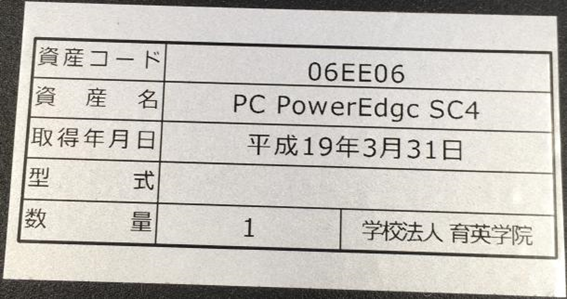
\includegraphics[keepaspectratio, scale=0.45]{gaiyo_1}
\caption{サレジオ高専にて用いられている備品シール}
\end{center}

\begin{center}
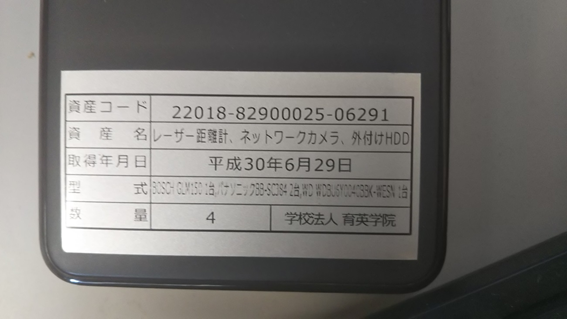
\includegraphics[keepaspectratio, scale=0.45]{gaiyo_2}
\caption{複数の備品が1つの資産コードにある備品シール}
\end{center}

\begin{center}
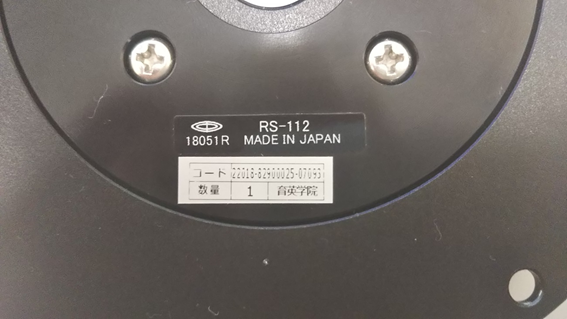
\includegraphics[keepaspectratio, scale=0.45]{gaiyo_3}
\caption{資産名が存在しない備品シール}
\end{center}

\end{figure}

サレジオ高専では現在,図1,図2,図3のような備品シールを用いて備品を管理している.
これらの資産コードと資産名,数量,管理者,管理場所の情報を整理し,管理を行う.

  \section{動作環境}
本ソフトウェアはWindows上での動作とAndroid上での動作の両方を行うことができる.Androidアプリケーションの作成はAndroid Javaを使用し,Windowsアプリケーションの作成はJavaを使用する.

  \section{前提条件}
  \noindent
1)本ソフトウェアはサレジオ高専所属宇都木修一先生が使用するものである.
\\2)上記の図1,図2,図3に記した備品シールそのものへの細工は不可とする.しかし備品シール外の場所への細工は可とする.
\\3)タブレットを用いる場合英数字およびコンボボックス等の選択形式のものを基本とする.
\\4)Android端末は普段持ち歩かず備品リスト等で現状の備品の確認を行うときにのみ使用する.
\\5)Android端末はインターネット接続が行えないものと考える.

  \section{デザイン要求}
  能動的に操作が可能なデザイン.1つの機能を利用するために複数の操作が必要となるシステムは避ける.

  \section{ソフトウェア構成}
  本ソフトウェアでは図1,図2,図3のような備品シールに記載されている,資産コード,資産名,数量,さらにその備品の管理者といった情報を整理し,Windowsでは新規情報の登録,登録情報の閲覧,また登録情報の所有者情報の変更の際や破損した際の編集も行い,Androidでは登録情報の閲覧を行う.
  
  また,備品の管理を簡易化するために各部屋ごとの備品といった検索機能や備品があるかどうかのチェック機能も搭載されている.

  \newpage
  \section{各種機能説明}
  \subsection{登録情報概要}
  情報の登録を行う際に使用する情報を以下に記す.
  \\1)資産コード
  \begin{figure}[h]
  \begin{center}
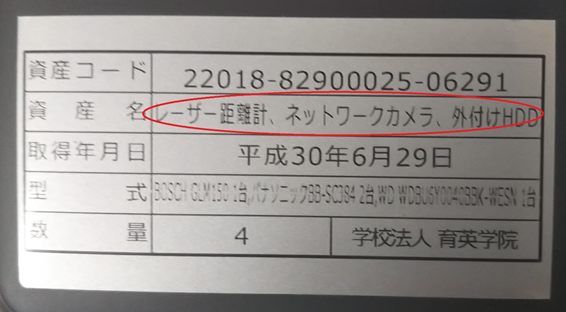
\includegraphics[keepaspectratio, scale=0.45]{jouhoutouroku1}
\caption{1つの資産コード内で複数の資産名を持つ備品シール}
\end{center}
\end{figure}
\\各備品シールに割り当てられている資産コード.図4のような複数個資産名が存在する場合は-1,-2などを資産コード末尾に入力して別の資産扱いで登録する.
\\2)資産名
\\備品の名称.図4のような場合には1つの資産コードに複数個をまとめて登録するのではなく-1,-2などを末尾につけた資産コードごとに登録する.
\\3)数量
  \begin{figure}[h]
  \begin{center}
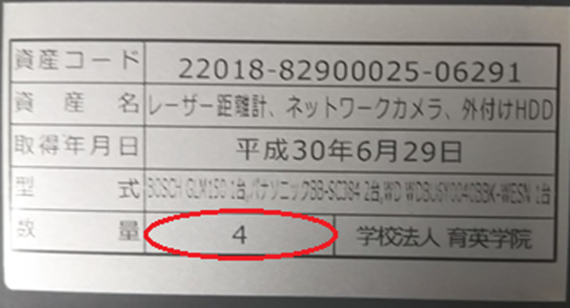
\includegraphics[keepaspectratio, scale=0.45]{jouhoutouroku3}
\caption{数量が明示されている備品シール}
\end{center}
\end{figure}
\\同資産コードを割り当てられた備品の数量.図5のように記載されている.
\\4)管理者
\\備品の管理者.
\\5)管理場所
\\資産コードの割り当てられている備品の管理場所.
  \newpage
  \begin{figure}[h]
    \begin{center}
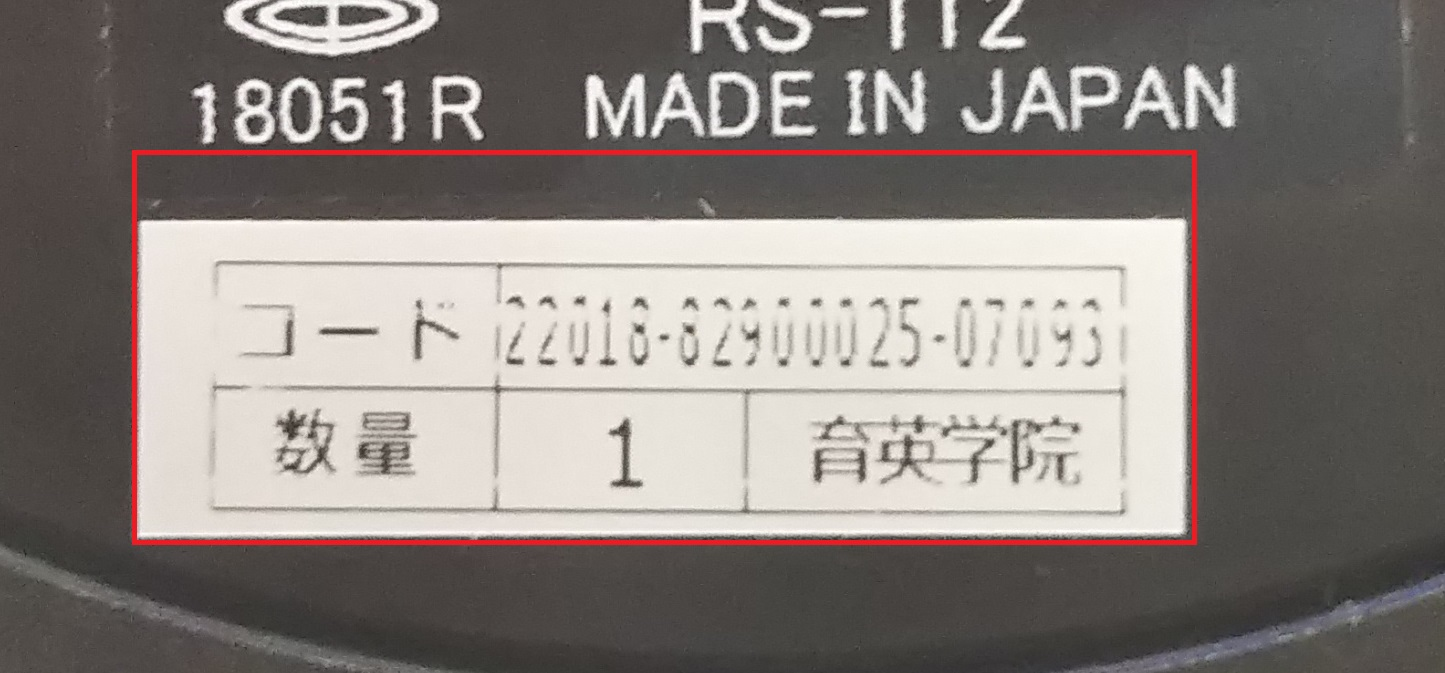
\includegraphics[keepaspectratio, scale=0.2]{jouhoutouroku2}
\caption{情報の備品シール}
\end{center}
\end{figure}

しかし図6の備品シールに資産名が存在しない場合のように備品シールの情報に欠落がある場合がある.この時,備品シールに掲載されていない情報は登録の際入力しないものとする.

  \subsection{システム概要}
  
システムの概要を以下に記す.windows及びandroidの両方で動作が同様のものはまとめて記載する.

\subsubsection{Windowsでの登録}
\noindent
1)アプリケーション起動後新規登録ボタンを押すことで新規登録ページが起動する.
\\2)新規登録ページに登録情報(資産コード,資産名,管理者,管理場所,数量)を入力.
 この時資産コード,管理者,管理場所は入力を必須とし,入力されていない場合は登録を行うことができない.それ以外である資産名,数量は備品シールに記載されていない場合があるため入力は任意とし,空欄でも登録が可能である.数量は数字(半角)でのみ入力可能とし,空欄なら可能であるが数字(半角)以外の文字が入力されている場合は上記入力必須項目が満たされていたとしても登録を行うことができない.
\\3)登録ボタンを押すことで入力した情報を確認するページが起動する.\\
 上記新規登録ページで入力が行われなかった場所には「入力されていません」が挿入される.

\subsubsection{Windowsでの検索}
\noindent
1)検索ボックスより場所や所有者などの検索を行いたい対象を選択する
\\2)隣接するコンボボックスがそれに対応した選択肢に変化する
\\3)変化した選択肢内から検索対象を選択,選択肢内に無い場合は手動で入力する.1)で他の検索対象を選択した場合も同様の操作を行う.
\\4)検索した対象が表に出力される

\subsubsection{Windowsでの表への表示}
\noindent
1)初期状態は空欄である
\\2)検索を行うことによって表示が行われる

\subsubsection{Windowsでの備品チェック}
\noindent
1)チェック用のボタンを操作する
\\2)表にチェックマークが出現する
\\3)チェックマークをつけた日の日付が表に更新され表示される.
\\4)チェックが完了次第,チェックマークを外す
\\5)終了ボタンを押すことでチェックモードが終了する

\subsubsection{Windowsでの編集}
\noindent
1)表に表示されている編集したい項目を選択
\\2)その中の編集したい情報の場所をダブルクリックすることで直接編集を行うことができる

\subsubsection{Windowsでの削除}
\noindent
1)表示されている削除したい項目を選択
\\2)その中の削除を選択する
\\3)確認後に削除を行う

\subsubsection{Androidでの表への表示}
\noindent
1)初期状態は登録されている項目の資産コードと最終確認日時がリストに表示されている
\\2)検索を行うことで検索結果のみを表示する
\\3)調べたい項目を選択するとダイアログに選択した項目の情報(資産コード,資産名,管理者,管理場所,個数,最終確認日)が表示される

\subsubsection{Androidでの検索(カテゴリ別)}
\noindent
1)ホーム画面の閲覧モードのボタンを操作する
\\2)画面が切り替わる
\\3)画面上部のにあるスピナーのうち左側のスピナーを操作する
\\4)画面中央に「ALL」,「場所」、「管理者」と表示され,上部に「項目を選択してください」と表示される
\\5)表示されている項目のうち検索したい項目を選択する
\\6)選択すると隣接しているスピナーが選択した項目に対応した項目に変化する
\\7)変化した項目から検索対象を選択,4)で「ALL」以外の項目を選択した場合も同様の操作を行う
\\8)検索対象がリストに出力される
\\9)4)で「ALL」を選択した場合はcsvファイルに保存されている全ての情報がリストに表示される

\subsubsection{Androidでの検索(直接入力)}
\noindent
{閲覧モードの場合}
\\1)ホーム画面の閲覧モードのボタンを操作する
\\2)画面が切り替わる
\\3)画面上部にある「資産コードを入力してください」と記載されている部分を選択する
\\4)キーボードが表示されるので検索したい資産コードを入力する
\\5)入力が終了したら右側にある検索ボタンを操作する
\\6)リストに入力された資産コードと一致する項目が表示される
\\7)何も入力していない時に検索ボタンを操作した場合リストにすべての情報が表示される
\noindent
\\
{チェックモードの場合}
\\1)ホーム画面のチェックモードのボタンを操作する
\\2)画面が切り替わる
\\3)画面上部にある「資産コードを入力してください」と記載されている部分を選択する
\\4)キーボードが表示されるので検索したい資産コードを入力する
\\5)入力が終了したら右側にある検索ボタンを操作する
\\6)リストに入力された資産コードと一致する項目が表示される
\\7)何も入力していない時に検索ボタンを操作した場合リストにすべての情報が表示される

\subsubsection{Androidでの備品チェック}
\noindent
1)ホーム画面のチェックモードと書かれたボタンを操作する
\\2)画面が切り替わる
\\3)チェックしたいリストの項目を選択する
\\4)項目の背景の色が変化する
\\5)ダイアログに選択した項目の情報(資産コード,資産名,管理者,管理場所,個数,最終確認日)が表示される
\\6)確認ボタンを押すと「チェックされました」と表示され,年と月が更新されcsvファイルに保存される
\\7)中断ボタンを押すと「中断しました」と表示され,csvファイルに書き込まれない
\\8)チェックモードを離れるとcsvファイルが出力される

  \newpage
  \section{更新経歴}
  \noindent
  2019/06/13 初期版作成	廣瀬 水間
  \\2019/06/28 誤字脱字修正,情報の修正 廣瀬
  \\2019/08/01 誤字脱字修正,不足情報修正,空白の削除,カンマの統一 水間 桶本
  \\2019/10/25 仕様変更に伴う修正 水間
 \\2019/11/28 仕様変更による大幅な修正 桶本
 \\2019/12/12 不足情報修正 桶本
\end{document}
